\documentclass[xcolor={svgnames}]{beamer}

% Layout (you can change theme and color scheme if you like)
\usetheme{Warsaw}
\usecolortheme{beaver}

% Language and math
\usepackage[utf8]{inputenc}
\usepackage[english]{babel}
\usepackage{amsmath,amssymb}
\usepackage{graphicx}
\usepackage{tikz}

\title{5G Networks and Signal Propagation}
\author{Lobov Mikhail}
\institute{RUDN University}
\date{\today}

\begin{document}

% ----------------------------------------
\begin{frame}
  \titlepage
\end{frame}
% ----------------------------------------

\begin{frame}{What is 5G?}
  \begin{block}{Short overview}
    \begin{itemize}
      \item<1-> 5G is the next generation of mobile networks.
      \item<2-> It uses higher carrier frequencies
        (for example around \(3.5\,\text{GHz}\) and above).
      \item<3-> Goals: higher data rates, lower latency,
        and support for a huge number of devices (IoT).
    \end{itemize}
  \end{block}

  \pause

  \begin{block}{Role of base stations (towers)}
    \begin{itemize}
      \item<4-> Cells become smaller in size, but there are many more of them.
      \item<5-> To cover a city, we need a dense deployment of base stations.
    \end{itemize}
  \end{block}
\end{frame}
% ----------------------------------------

\begin{frame}{Signal propagation in 5G}
  \begin{block}{Basic idea}
    The radio signal from the base station to the user attenuates along the path:
    \[
      P_{\text{rx}} \propto \frac{1}{d^{\alpha}},
    \]
    where \(d\) is the distance to the base station and \(\alpha \approx 2\text{--}4\)
    is the path loss exponent.
  \end{block}

  \pause

  \begin{block}{Features of high frequencies}
    \begin{itemize}
      \item<2-> Stronger absorption by walls and other obstacles.
      \item<3-> Harder to cover large areas with a single tower.
      \item<4-> \alert{Line-of-sight} (LoS) becomes very important.
    \end{itemize}
  \end{block}
\end{frame}
% ----------------------------------------

\begin{frame}{Noise and signal-to-noise ratio}
  \begin{block}{Noise}
    \begin{itemize}
      \item<1-> Thermal noise in the receiver.
      \item<2-> Interference from electronics and other devices.
    \end{itemize}
  \end{block}

  \pause

  \begin{block}{Signal-to-noise ratio (SNR)}
    \uncover<3->{The link quality is often described by}
    \[
      \uncover<3->{\text{SNR}
        = \frac{P_{\text{signal}}}{P_{\text{noise}}}.}
    \]

    \uncover<4->{The larger \(\text{SNR}\), the more reliably we can transmit data.}
    \uncover<5->{When \(\text{SNR}\) is small, the error probability increases
      and we have to reduce the data rate.}
  \end{block}
\end{frame}
% ----------------------------------------

\begin{frame}{Interference in a cellular network}
  \frametitle{Interference in a cellular network}

  \begin{columns}
    \begin{column}{0.55\textwidth}
      \begin{block}{Sources of interference}
        \begin{itemize}
          \item<1-> Neighboring cells using the same or nearby frequencies.
          \item<2-> Other users inside the same cell.
          \item<3-> Reflections from buildings (\alert{multipath} propagation).
        \end{itemize}
      \end{block}

      \pause

      \begin{block}{Effect}
        \uncover<4->{The sum of all signals can both strengthen and weaken
        the useful signal.}
        \uncover<5->{This leads to deep fades of the received power and
        bit errors.}
      \end{block}
    \end{column}

    \begin{column}{0.45\textwidth}
      % Replace this with your own image of a 5G network if you like
      \begin{center}
        \uncover<2->{
          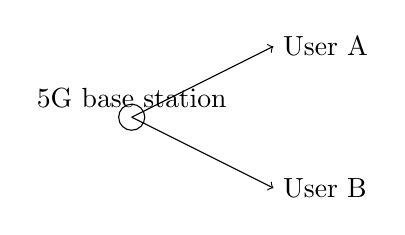
\begin{tikzpicture}[scale=0.9]
            \draw (0,0) node[circle,draw] {} node[above]{5G base station};
            \draw[->] (0,0) -- (2,1) node[right]{User A};
            \draw[->] (0,0) -- (2,-1) node[right]{User B};
          \end{tikzpicture}
        }
      \end{center}
      % Or, for example:
      % \uncover<2->{
      %   \includegraphics[width=\textwidth]{5g_cells_example}
      % }
    \end{column}
  \end{columns}
\end{frame}
% ----------------------------------------

\begin{frame}{Mitigating noise and interference}
  \begin{enumerate}
    \item \uncover<1->{\alert{Multiple access and scheduling} \\
      Careful allocation of frequencies and time slots between cells and users.}
    \item \uncover<2->{\alert{MIMO and beamforming} \\
      Using multiple antennas to form narrow beams towards a specific user.}
    \item \uncover<3->{\alert{Small cells} \\
      Many small base stations, shorter distances, better \(\text{SNR}\).}
    \item \uncover<4->{\alert{Adaptive modulation and coding} \\
      With high \(\text{SNR}\) we use high data rates; with low \(\text{SNR}\)
      we switch to more robust schemes.}
  \end{enumerate}
\end{frame}
% ----------------------------------------

\begin{frame}{Summary}
  \begin{block}{Key ideas}
    \begin{itemize}
      \item<1-> 5G uses higher frequencies, so the signal attenuates more
        and is more sensitive to obstacles.
      \item<2-> Link quality is determined by noise and interference
        (through \(\text{SNR}\)).
      \item<3-> To cope with these problems we use MIMO, beamforming,
        small cells and smart radio resource management.
    \end{itemize}
  \end{block}

  \uncover<4->{
    \vspace{0.5cm}
    \centering
    \alert{Idea for improvement: add real numbers for data rates and carrier
    frequencies of a concrete operator.}
  }
\end{frame}
% ----------------------------------------

\end{document}
